\documentclass[11pt,a4paper,titlepage]{article}
\usepackage[a4paper]{geometry}
\usepackage[utf8]{inputenc}
\usepackage[english]{babel}
\usepackage{lipsum}

\usepackage{amsmath, amssymb, amsfonts, amsthm, fouriernc, mathtools}
% mathtools for: Aboxed (put box on last equation in align envirenment)
\usepackage{microtype} %improves the spacing between words and letters

\usepackage{graphicx}
\graphicspath{ {./pics/} {./eps/}}
\usepackage{epsfig}
\usepackage{epstopdf}

%%%%%%%%%%%%%%%%%%%%%%%%%%%%%%%%%%%%%%%%%%%%%%%%%%
%% COLOR DEFINITIONS
%%%%%%%%%%%%%%%%%%%%%%%%%%%%%%%%%%%%%%%%%%%%%%%%%%
\usepackage[svgnames]{xcolor} % Enabling mixing colors and color's call by 'svgnames'
%%%%%%%%%%%%%%%%%%%%%%%%%%%%%%%%%%%%%%%%%%%%%%%%%%
\definecolor{MyColor1}{rgb}{0.2,0.4,0.6} %mix personal color
\newcommand{\textb}{\color{Black} \usefont{OT1}{lmss}{m}{n}}
\newcommand{\blue}{\color{MyColor1} \usefont{OT1}{lmss}{m}{n}}
\newcommand{\blueb}{\color{MyColor1} \usefont{OT1}{lmss}{b}{n}}
\newcommand{\red}{\color{LightCoral} \usefont{OT1}{lmss}{m}{n}}
\newcommand{\green}{\color{Turquoise} \usefont{OT1}{lmss}{m}{n}}
%%%%%%%%%%%%%%%%%%%%%%%%%%%%%%%%%%%%%%%%%%%%%%%%%%




%%%%%%%%%%%%%%%%%%%%%%%%%%%%%%%%%%%%%%%%%%%%%%%%%%
%% FONTS AND COLORS
%%%%%%%%%%%%%%%%%%%%%%%%%%%%%%%%%%%%%%%%%%%%%%%%%%
%    SECTIONS
%%%%%%%%%%%%%%%%%%%%%%%%%%%%%%%%%%%%%%%%%%%%%%%%%%
\usepackage{titlesec}
\usepackage{sectsty}
%%%%%%%%%%%%%%%%%%%%%%%%
%set section/subsections HEADINGS font and color
\sectionfont{\color{MyColor1}}  % sets colour of sections
\subsectionfont{\color{MyColor1}}  % sets colour of sections

%set section enumerator to arabic number (see footnotes markings alternatives)
\renewcommand\thesection{\arabic{section}.} %define sections numbering
\renewcommand\thesubsection{\thesection\arabic{subsection}} %subsec.num.

%define new section style
\newcommand{\mysection}{
\titleformat{\section} [runin] {\usefont{OT1}{lmss}{b}{n}\color{MyColor1}} 
{\thesection} {3pt} {} } 

%%%%%%%%%%%%%%%%%%%%%%%%%%%%%%%%%%%%%%%%%%%%%%%%%%
%		CAPTIONS
%%%%%%%%%%%%%%%%%%%%%%%%%%%%%%%%%%%%%%%%%%%%%%%%%%
\usepackage{caption}
\usepackage{subcaption}
%%%%%%%%%%%%%%%%%%%%%%%%
\captionsetup[figure]{labelfont={color=Turquoise}}

%%%%%%%%%%%%%%%%%%%%%%%%%%%%%%%%%%%%%%%%%%%%%%%%%%
%		!!!EQUATION (ARRAY) --> USING ALIGN INSTEAD
%%%%%%%%%%%%%%%%%%%%%%%%%%%%%%%%%%%%%%%%%%%%%%%%%%
%using amsmath package to redefine eq. numeration (1.1, 1.2, ...) 
%%%%%%%%%%%%%%%%%%%%%%%%
\renewcommand{\theequation}{\thesection\arabic{equation}}

%set box background to grey in align environment 
\usepackage{etoolbox}% http://ctan.org/pkg/etoolbox
\makeatletter
\patchcmd{\@Aboxed}{\boxed{#1#2}}{\colorbox{black!15}{$#1#2$}}{}{}%
\patchcmd{\@boxed}{\boxed{#1#2}}{\colorbox{black!15}{$#1#2$}}{}{}%
\makeatother
%%%%%%%%%%%%%%%%%%%%%%%%%%%%%%%%%%%%%%%%%%%%%%%%%%




%%%%%%%%%%%%%%%%%%%%%%%%%%%%%%%%%%%%%%%%%%%%%%%%%%
%% DESIGN CIRCUITS
%%%%%%%%%%%%%%%%%%%%%%%%%%%%%%%%%%%%%%%%%%%%%%%%%%
\usepackage[siunitx, american, smartlabels, cute inductors, europeanvoltages]{circuitikz}
%%%%%%%%%%%%%%%%%%%%%%%%%%%%%%%%%%%%%%%%%%%%%%%%%%



\makeatletter
\let\reftagform@=\tagform@
\def\tagform@#1{\maketag@@@{(\ignorespaces\textcolor{red}{#1}\unskip\@@italiccorr)}}
\renewcommand{\eqref}[1]{\textup{\reftagform@{\ref{#1}}}}
\makeatother
\usepackage{hyperref}
\hypersetup{colorlinks=true}

%%%%%%%%%%%%%%%%%%%%%%%%%%%%%%%%%%%%%%%%%%%%%%%%%%
%% PREPARE TITLE
%%%%%%%%%%%%%%%%%%%%%%%%%%%%%%%%%%%%%%%%%%%%%%%%%%
\title{\blue Introduction to Electrical Engineering 2 \\
\blueb Assignment Solution $1$}
\author{Igor Shevtsov}
\date{\today}
%%%%%%%%%%%%%%%%%%%%%%%%%%%%%%%%%%%%%%%%%%%%%%%%%%



\begin{document}
\maketitle

\section{Question 1 Solution}{%
\subsection{Section 1}{Following equations describe current-voltage relations between some%
\footnote{Resistor, Capacitor and Inductor} circuit elements:%
\begin{align}
v_R&=iR \label{eq:1} \\
i_C&=C\dot{v}_C \label{eq:2} \\
v_L&=L\dot{i}_L \label{eq:3}
\end{align}
Applying nodal method at the $v_L$ node of circuit on Figure~\ref{fig:q1fig}
\begin{align}
I_0=\dfrac{v_L}{R}+i_L  \label{eq:4}
\end{align}
Using \eqref{eq:3} one could obtain a differential equation
\begin{align}
\Aboxed{\dot{i_L}(t)+\tfrac{R}{L}i_L(t)&=\tfrac{R}{L}I_0 \quad,\, t>0} \label{eq:5}
\end{align}
%%%%%%%%%%%%%%%%%%%%%%%%%%%%%%%%%%%%%%%%%%%%%%%%%%
%%%%%%%%%%%%%%%%%%%%%%%%%%%%%%%%%%%%%%%%%%%%%%%%%%
\ctikzset {bipoles/length=1.2cm}
\begin{figure}[!htb]
\centering
\begin{circuitikz}[scale =1.2]\draw
(0,0) to [current source = $I_0$] (0,2) -- (2,2)
node[anchor=south] {$v_L$}
to [R, l_= $R$, i>^=$i_R(t)$, *-] (2,0)
 (2,2) -- (4,2) to [L=$L$, i>^=$i_L(t)$, v=$v_L(t)$] (4,0) -- (0,0)
;\end{circuitikz}
\caption{\green Electric Circuit}
\label{fig:q1fig}
\end{figure}
}\label{sub:sub1}
%%% END UBSECTION 1 %%%%%%%%%%%%%%%%%%%%%%%%%%%%%%%%%%%%%%
\subsection{Section 2}{
Assuming steady state yields constant\footnote{Resistor Shortened by Inductor} current, therefore
\begin{align}
\textsl{ZSR:\quad} \Aboxed{i_L&=I_0 \label{eq:6}}
\end{align}
\begin{proof}
Solving ZIR of the equation~\eqref{eq:5} :
\begin{align}
i_{L,ZIR}(t)=A\exp({\dfrac{-t}{\tau}})\label{eq:7}\\
\lim_{t \to \infty}i_{L}(t)=\lim_{t \to \infty}\left(i_{L, ZIR}+i_{L,ZSR}\right)=i_{L, ZSR}=I_0 \nonumber
\end{align}
\end{proof}
}\label{sub:sub2}%
%%% END SUBSECTION 2 %%%%%%%%%%%%%%%%%%%%%%%%%%%%%%%%%%%%%
\subsection{Section 3}{
Summarizing equation~\eqref{eq:6} with \eqref{eq:7} and activating given initial condition $i_L(t=0)=2~\si{\A}$ results in final solution $i_L(t)$, where $\tau=\frac{L}{R}$:
\begin{align*}
\Aboxed{i_{L}(t)=I_0+\left(2- I_0\right)exp\left({\dfrac{-t}{\tau}}\right) \quad, t>0}
\end{align*}
\begin{figure}[!htb]
\centering
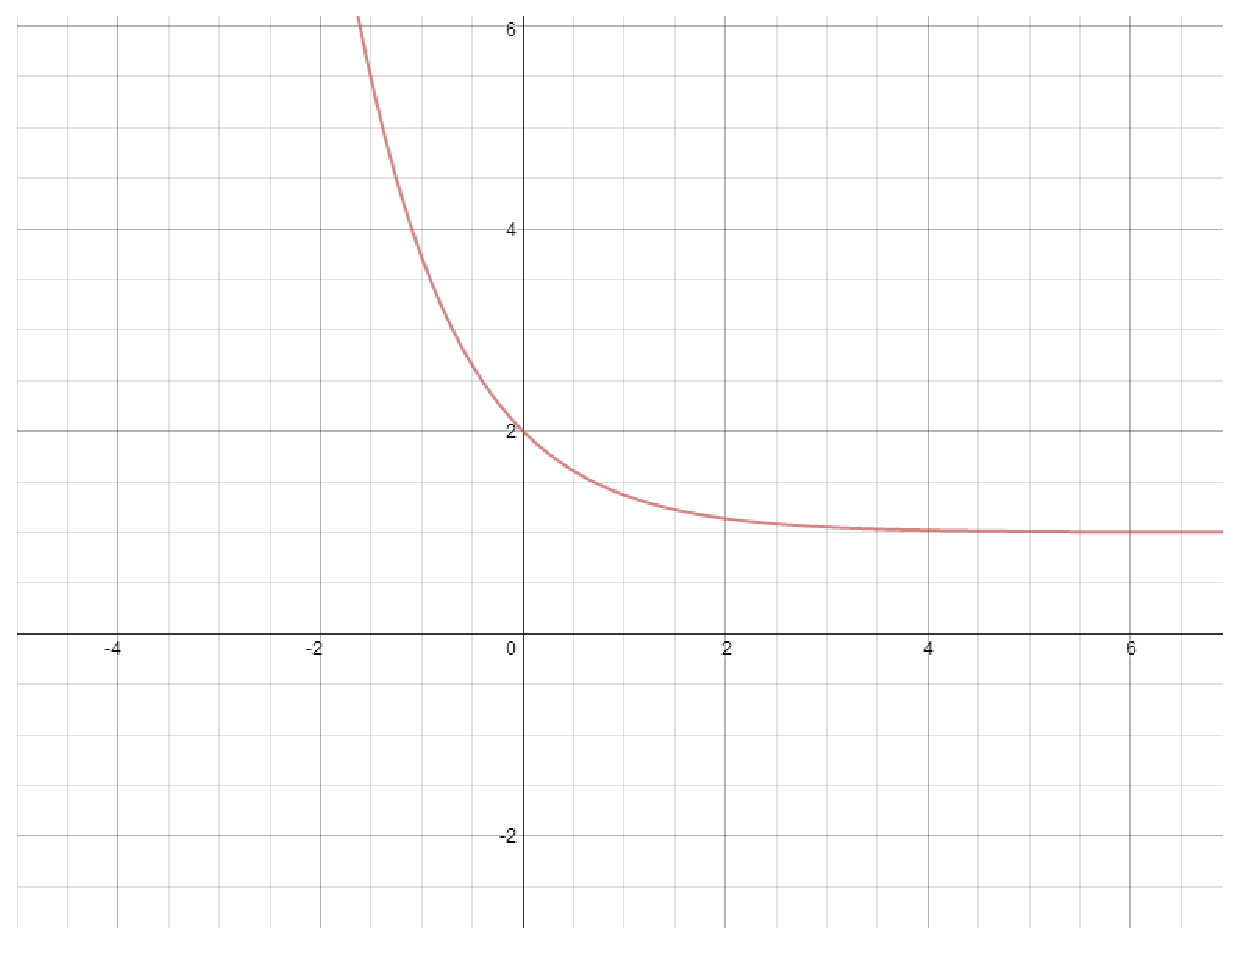
\includegraphics[scale=.3]{fig2.eps}
\caption{\green Inductor Current with $I_0=1A$}
\label{fig:q1fig2}
\end{figure}
}\label{sub:sub3}
%%% END SUBSECTION 3 %%%%%%%%%%%%%%%%%%%%%%%%%%%%%%%%%%%%%
}\label{sec:q1sec}
%%% END SECTION 1 %%%%%%%%%%%%%%%%%%%%%%%%%%%%%%%%%%%%%%%



\section{Question 2 Solution}{
\subsection{Section 1}{
Consider circuit on Figure~\ref{fig:q2fig1b}. Now\footnote{Inductor is Short} applying current divider technique one could easily calculate the following currents:\par
\begin{align*}
i_1 = \dfrac{40}{500+2k||6k}\cdot\dfrac{2k}{500+2k||6k}\\ \\
i_2 = \dfrac{40}{500+2k||6k}\cdot\dfrac{6k}{500+2k||6k}\\ \\
\Aboxed{i_1(0^-)=20\,\si{mA} \qquad i_2(0^-)=60\,\si{mA}}
\end{align*}
%%%%%%%%%%%%%%%%%%%%%%%%%%%%%%%%%%%%%%%%%%%%%%%%%%
\ctikzset {bipoles/length=.8cm}
\begin{figure}[!htb]
\centering
\begin{subfigure}{.5\textwidth}
\begin{circuitikz}[scale =.6]\draw
(0,0) to [voltage source = $40\,\si{\volt}$] (0,3)
to [R = $500~\si{\ohm}$] (2,3)
to [opening switch, l_= {t>0}] (3,3) -- (4,3)
node[anchor=south]{$v_x$}
to [R = $6~\si{\kohm}$, i>_=$i_1$, *-] (7,3)
to [L, l_= $400~\si{m\henry}$] (7,0) -- (0,0)
(4,3) to [R, l_= $2~\si{\kohm}$, i>_=$i_2$] (4,0)
;\end{circuitikz}
\caption{\green \,Superposed Circuit}
\label{fig:q2fig1a}
\end{subfigure}
\begin{subfigure}{.5\textwidth}
\begin{circuitikz}[scale =.6]\draw
(0,0) to [voltage source = $40\,\si{\volt}$] (0,3)
to [R = $500~\si{\ohm}$] (2,3) -- (4,3)
to [R = $6~\si{\kohm}$, i>_=$i_1$] (6,3)
to [L, l_= $400~\si{m\henry}$] (6,0) -- (0,0)
(3,3) node[anchor=south]{$v_x$}
to [R, l_= $2~\si{\kohm}$, i>_=$i_2$,*-] (3,0)
;\end{circuitikz}
\caption{\green \,Past Time Circuit}
\label{fig:q2fig1b}
\end{subfigure}
\begin{subfigure}{.4\textwidth}
\begin{circuitikz}[scale =.6]\draw
(0,0) to [R = $8\,\si{\kohm}$, i_<=$i_2$,-*] (0,3) -- (2,3) 
node[anchor=south]{$v_L$}
to [L = $400\,\si{m\henry}$, i>^=$i_1$,*-] (2,0) -- (0,0)
;\end{circuitikz}
\caption{\green \,Future Time Circuit}
\label{fig:q2fig1c}
\end{subfigure}
\caption{\green Question 2 Circuit}
\label{fig:q2fig1}
\end{figure}
}
%%% END SUBSECTION 1 %%%%%%%%%%%%%%%%%%%%%%%%%%%%%%%%%%%%%%
\subsection{Section 2}{
Assuming continuity in the inductor current $i_1(0^-)=i_1(0^+)=20\,\si{\mA}$ on Figure~\ref{fig:q2fig1c}, where $i_1=-i_2$, thus, setting $i_1(0^+)=-i_2(0^+)=20\,\si{\mA}$ we get the currents
\begin{align*}
\Aboxed{i_1(0^+)=20\,\si{mA} \qquad i_2(0^+)=-20\,\si{\mA}}
\end{align*}
}
%%% END SUBSECTION 2 %%%%%%%%%%%%%%%%%%%%%%%%%%%%%%%%%%%%%%
\subsection{Section 3}{It's obvious, that circuits \ref{fig:q2fig1b} and \ref{fig:q2fig1c} are equivalent to Figure~\ref{fig:q1fig} (Page~\pageref{fig:q1fig}) with $\tau=50~\si{\ms}$ and $I_0=V_0/R_{eq}=20~\si{\mA}$:
\begin{align}
\Aboxed{\dot{i_L}(t)+\tfrac{R}{L}i_L(t)&=\tfrac{R}{L}I_0 \quad,\, t>0}
\end{align}
}
%%% END SUBSECTION 3 %%%%%%%%%%%%%%%%%%%%%%%%%%%%%%%%%%%%%%
\subsection{Section 4}{Again, adopting ZIR\footnote{Since, there is no source in the circuit} solution~\eqref{eq:7} 
\begin{align*}
\Aboxed{i_1(t)&=i_1(0^+)\exp\left({\dfrac{-t}{\tau}}\right) \quad, t>0} \\ \label{eq:8}
\Aboxed{i_2(t)&=-i_1(t)}
\end{align*}
}
%%% END SUBSECTION 3 %%%%%%%%%%%%%%%%%%%%%%%%%%%%%%%%%%%%%%
}\label{sec:q2sec}
%%% END SECTION 2 %%%%%%%%%%%%%%%%%%%%%%%%%%%%%%%%%%%%%%%%



\section{Question 3 Solution}{
\subsection{Section 1}{
\ctikzset {bipoles/length=.8cm}
\begin{figure}[!htb]
\begin{subfigure}{\textwidth}
\begin{circuitikz}[scale =.8]\draw
(0,0) to [current source = $15\,\si{\mA}$] (0,3) -- (2,3)
to [R, l= $2.4\,\si{\kohm}$] (2,0) -- (4,0)
to [C,l_=$0.25\,\si{\micro\farad}$] (4,2.5)
to[short, -o](3.3,3.3)
(4,3)node[anchor=south]{t=0}
node[ocirc] (A) at (3,3) {}
node[ocirc] (B) at (5,3) {}
(B) to [open, v=${}$] (A)
(5,3)to[short, o-](6,3)--(6,5)
to [R=$25\,\si{\kohm}$] (8,5)--(8,3)
to [cI,l_=$\alpha \cdot v_{\phi}$] (6,3)
(2,3)to[short,-o](3,3)
(8,3)--(9,3)
to [R, l_= $15~\si{\kohm}$,v^=$v_{\phi}$] (9,0) -- (0,0)
;\end{circuitikz}
\caption{\green \,Superposed Circuit}
\label{fig:q3fig1a}
\end{subfigure}
\begin{subfigure}{.5\textwidth}
\begin{circuitikz}[scale =1]\draw
(0,0) to [current source = $15~\si{\mA}$] (0,2) -- (2,2)
node[anchor=south] {$v_L$}
to [R, l_= $2.4~\si{\kohm}$] (2,0)
 (2,2) -- (4,2) to [C, l_=$0.25~\si{\micro\farad}$] (4,0) -- (0,0)
;\end{circuitikz}
\caption{\green \,Past Time Circuit}
\label{fig:q3fig1b}
\end{subfigure}
\begin{subfigure}{.4\textwidth}
\begin{circuitikz}[scale =.65]\draw
(0,0) to [C, l_= $0.25~\si{\micro\farad}$] (0,3)--(2.7,3)--(2.7,4.5) 
to [R, l_= $25~\si{\kohm}$] (6.5,4.5)--(6.5,2.2)
to [cI, l= $\alpha \cdot v_{\phi}$] (2.7,2.2)--(2.7,3)
(6.5,3)--(8,3) to [R, l_= $15~\si{\kohm}$] (8,0)--(0,0)
;\end{circuitikz}
\caption{\green \,Future Time Circuit}
\label{fig:q3fig1c}
\end{subfigure}
\caption{\green Question 3 Circuit}
\label{fig:q3fig1}
\end{figure}
%%%%%%%%%%%%%%%%%%%%%%%%%%%%%%%%%%%%%%%%%%%%%%%%%%
}
%%% END SUBSECTION 1 %%%%%%%%%%%%%%%%%%%%%%%%%%%%%%%%%%%%%%
\subsection{Section 2}{
}
%%% END SUBSECTION 2 %%%%%%%%%%%%%%%%%%%%%%%%%%%%%%%%%%%%%%
\subsection{Section 3}{
}
%%% END SUBSECTION 3 %%%%%%%%%%%%%%%%%%%%%%%%%%%%%%%%%%%%%%
\subsection{Section 4}{
}
%%% END SUBSECTION 4 %%%%%%%%%%%%%%%%%%%%%%%%%%%%%%%%%%%%%%
}\label{sec:q3sec}
%%% END SECTION 3 %%%%%%%%%%%%%%%%%%%%%%%%%%%%%%%%%%%%%%%



\end{document}